\documentclass[tikz,border=2pt]{standalone}
\usepackage{tikz,pgfplots,pgf}
\usetikzlibrary{decorations.pathmorphing,decorations.text,calc,snakes}
\newcommand{\MYPI}{3.14159}
\newcommand{\MYTHETA}{33}
\newcommand{\MYSCALE}{3}
\newcommand{\XSHIFT}{0}
\newcommand{\OPRIME}{0}
\newcommand{\LINEPT}{3pt}
\DeclareMathSizes{20}{30}{20}{20} 
\definecolor{myblue}{rgb}{0.0,0.447,0.741}
\definecolor{myblue2}{rgb}{0.301,0.745,0.933}
\definecolor{myorange}{rgb}{0.85,0.325,0.098}
\definecolor{mygreen}{rgb}{0.466,0.674,0.188}
\definecolor{mypurple}{rgb}{0.494,0.184,0.556}
\definecolor{myred}{rgb}{0.635,0.078,0.184}
\definecolor{myyellow}{rgb}{0.929,0.694,0.125}
\begin{document}
	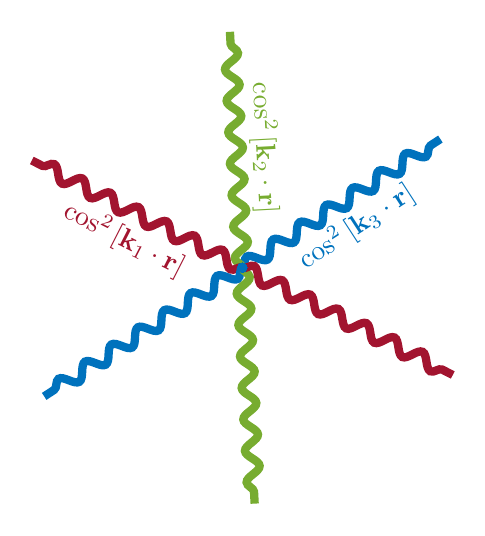
\begin{tikzpicture}\label{fig:k_vec}
	
		%%
			
%		\coordinate (o1) at (0,0) ;
%		\coordinate (g1) at ({1*\MYSCALE},0); 
%		\coordinate (g2) at ({0.5*\MYSCALE},{0.866*\MYSCALE}); 
%		\coordinate (g3) at ({0.5*\MYSCALE},{-0.866*\MYSCALE}); 
%		\coordinate (g4) at ({-0.5*\MYSCALE},{-0.866*\MYSCALE}); 
%		\coordinate (g5) at ({-0.5*\MYSCALE},{0.866*\MYSCALE}); 
%		\coordinate (g6) at ({-1*\MYSCALE},0); 
		
		\coordinate (o1) at (0,0) ;
		\coordinate (g1) at ({\MYSCALE*cos(\MYTHETA + 0)},{\MYSCALE*sin(\MYTHETA + 0)}); 
		\coordinate (g2) at ({\MYSCALE*cos(\MYTHETA + 60 )},{\MYSCALE*sin(\MYTHETA + 60)}); 
		\coordinate (g3) at ({\MYSCALE*cos(\MYTHETA + 120)},{\MYSCALE*sin(\MYTHETA + 120)}); 
		\coordinate (g4) at ({\MYSCALE*cos(\MYTHETA + 180)},{\MYSCALE*sin(\MYTHETA + 180)}); 
		\coordinate (g5) at ({\MYSCALE*cos(\MYTHETA + 240)},{\MYSCALE*sin(\MYTHETA + 240)}); 
		\coordinate (g6) at ({\MYSCALE*cos(\MYTHETA + 300)},{\MYSCALE*sin(\MYTHETA + 300)}); 
		
%		\draw[,decorate, decoration = {snake, segment length = .4cm},color=myblue,solid,line width=\LINEPT] (o1) -- (g1) node  [near end, below, sloped] (TextNode) {\color{myblue}$\mathbf{B}_{2}$};
%		\draw[,decorate, decoration = {snake, segment length = .4cm},color=mygreen,solid,line width=\LINEPT] (o1) -- (g2) node  [near end, above, sloped] (TextNode) {\color{mygreen}$\mathbf{B}_{1}$};
%		\draw[,decorate, decoration = {snake, segment length = .4cm},color=myred,solid,line width=\LINEPT] (o1) -- (g3) node  [near end, below, sloped] (TextNode) {\color{myred}$\mathbf{B}_{3}$};
%		\draw[,decorate, decoration = {snake, segment length = .4cm},color=mygreen,solid,line width=\LINEPT] (o1) -- (g4) node  [near end, above, sloped] (TextNode) {};
%		\draw[,decorate, decoration = {snake, segment length = .4cm},color=myred,solid,line width=\LINEPT] (o1) -- (g5) node  [near end, below, sloped] (TextNode) {};
%		\draw[,decorate, decoration = {snake, segment length = .4cm},color=myblue,solid,line width=\LINEPT] (o1) -- (g6) node  [near end, above, sloped] (TextNode) {};
		
		\draw[,decorate, decoration = {snake, segment length = .4cm},color=myblue,solid,line width=\LINEPT] (o1) -- (g1) node  [midway, below, sloped] (TextNode) {\color{myblue}$\cos^2\left[\mathbf{k}_3\cdot\mathbf{r}\right]$};
		\draw[,decorate, decoration = {snake, segment length = .4cm},color=mygreen,solid,line width=\LINEPT] (o1) -- (g2) node  [midway, above, sloped] (TextNode) {\color{mygreen}$\cos^2\left[\mathbf{k}_2\cdot\mathbf{r}\right]$};
		\draw[,decorate, decoration = {snake, segment length = .4cm},color=myred,solid,line width=\LINEPT] (o1) -- (g3) node  [midway, below, sloped] (TextNode) {\color{myred}$\cos^2\left[\mathbf{k}_1\cdot\mathbf{r}\right]$};
		\draw[,decorate, decoration = {snake, segment length = .4cm},color=myblue,solid,line width=\LINEPT] (o1) -- (g4) node  [near end, above, sloped] (TextNode) {};
		\draw[,decorate, decoration = {snake, segment length = .4cm},color=mygreen,solid,line width=\LINEPT] (o1) -- (g5) node  [near end, below, sloped] (TextNode) {};
		\draw[,decorate, decoration = {snake, segment length = .4cm},color=myred,solid,line width=\LINEPT] (o1) -- (g6) node  [near end, above, sloped] (TextNode) {};
		
		
		\draw[mark options={color=myblue},mark size=1.5\LINEPT] plot[mark=*] (o1);
		
		%%
		
%		\draw[dashed,->,color=myred,thick] (o2) -- (l1) node [midway, above, sloped] (TextNode) {$\mathbf{k_{22}}$};
%		\draw[dashed,->,color=myred,thick] (o2) -- (l2) node [midway, above, sloped] (TextNode)  {$\mathbf{k_{21}}$};
%		\draw[dashed,->,color=myred,thick] (o2) -- (l3) node [midway, above, sloped] (TextNode)  {$\mathbf{k_{23}}$};
%		\draw[mark options={color=myred},mark size=1pt] plot[mark=*] (o2);

	\end{tikzpicture}
\end{document}
